\documentclass[a4paper,12pt]{article}
\usepackage[utf8]{inputenc}
\usepackage{wrapfig}
\usepackage{graphicx}
\usepackage{float}
\usepackage{amsmath}
\usepackage{pslatex}
\usepackage[portuguese]{babel}
\usepackage{indentfirst}
\usepackage{natbib}
\usepackage{todonotes}
\usepackage{tikz}
\usepackage[lmargin=3cm,rmargin=3cm,tmargin=2.5cm,bmargin=2.5cm]{geometry}
\setlength{\parindent}{1cm}
\setlength{\baselineskip}{1.5cm}
\renewcommand{\contentsname}{Sumário}



\begin{document}

\begin{titlepage}
 \begin{center}
  { \large FUNDAÇÃO GETULIO VARGAS}\\[0.3cm]
  { \large ESCOLA DE MATEMÁTICA APLICADA}\\[0.5cm]
  { \large CURSO DE GRADUAÇÃO EM}\\[0.3cm]
  { \large MATEMÁTICA APLICADA}\\[0.3cm]
 
  \vspace{55 mm}

  {\bf \large Dinâmica de Disseminação de Notícias em}\\[0.1cm]
  {\bf \large Redes Complexas}\\[1.7cm]

  { por}\\[0.6cm]
  {\large Elisa Mussumeci}\\[0.1cm]


  \vspace{7cm}

  { Rio de Janeiro}\\[0.1cm]
  { 2015}\\[0.6cm]
  { FUNDAÇÃO GETÚLIO}\\[0.1cm]
  { VARGAS}\\[0.1cm]
 \end{center}
\end{titlepage}

\begin{titlepage}
 
 \begin{center}
  {\large FUNDAÇÃO GETULIO VARGAS}\\[0.3cm]
  {\large ESCOLA DE MATEMÁTICA APLICADA}\\[0.5cm]
  {\large CURSO DE GRADUAÇÃO EM}\\[0.3cm]
  {\large MATEMÁTICA APLICADA}\\[0.3cm]


  \vspace{20 mm}


  {\large Dinâmica de Disseminação de Notícias em}\\[0.1cm]
  {\large Redes Complexas}\\[2.5cm]

  
  \bf "Declaro ser o único autor do presente projeto de monografia que refere-se ao
plano de trabalho a ser executado para continuidade da monografia e ressalto
que não recorri a qualquer forma de colaboração ou auxílio de terceiros para
realizá-lo a não ser nos casos e para os fins autorizados pelo professor orientador"

  \vspace{3.5cm}


  \line(1,0){220}\\[0.1cm]
  {\bf Elisa Mussumeci}\\[2cm]
  {\bf Orientador: Flavio Codeço Coelho}\\[5cm]




  {Rio de Janeiro}\\[0.1cm]
  {2015}
 \end{center}
\end{titlepage}

\begin{titlepage}
 \begin{center}
 
  {\bf \large ELISA MUSSUMECI}\\[0.3cm]

  \vspace{25 mm}

  {\bf \large Dinâmica de Disseminação de Notícias em}\\[0.1cm]
  {\bf \large Redes Complexas}\\[4cm]

  {“Monografia apresentada à Escola de Matemática Aplicada}\\[0.1cm]
  {como requisito parcial para obtenção do grau de Bacharel }\\[0.1cm]
  {em Matemática Aplicada”}\\[6cm]


  {Aprovado em \ \line(1,0){20} \ \ de \line(1,0){62} \ \ de \line(1,0){30} \ .}\\[0.1cm]
  {Grau atribuido ao Projeto de Monografia: \line(1,0){20} \ . }\\[3cm]
  
  
  {\line(1,0){250}}\\
  {\bf Professor Orientador: Flávio Codeço Coelho}\\[0.1cm]
  {\bf Escola de Matemática Aplicada}\\[0.1cm]
  {\bf Fundação Getulio Vargas}
 \end{center}
\end{titlepage}

\newpage\null\thispagestyle{empty}\newpage

\tableofcontents

\pagebreak

\begin{abstract}
 
O processo de formação de opinião é fortemente influenciado pela mídia digital.
Entretanto pouco se sabe sobre o processo de disseminação de notícias e os fatores que determinam o alcance de cada
notícia.

A disseminação de uma notícia se dá por meio de um ou mais caminhos em uma rede desconhecida de influência entre 
formadores de opinião (produtores de notícias). Este padrão pode ser recuperado, com algum grau de incerteza, a partir de dados
da sequência temporal das publicações sobre um mesmo tema, e dos links nelas contidos.

Este projeto tem como objetivo caracterizar as redes de interligação de veículos de mídia e modelar a dinâmica do espalhamento 
de notícias, a fim de prever tendências e mapear questões de interesse.

\end{abstract}

\pagebreak

\section{Introdução}

Atualmente podemos considerar a internet como um dos principais meios de veiculação de notícias e informação. Com o crescente
número de pessoas aderindo à redes sociais, o compartilhamento de notícias aumentou sifnificamente, o que tornou fundamental
o papel das mídias digitais no acesso à informação.




A mídia tem um forte papel influenciador no processo de formação de opinião. Sendo assim, podemos considerar 
importante entender como uma notícia se comporta na mídia

A partir dos dados do Projeto Media Cloud Brasil, estudamos ccomo uma notícia se dissemina na mídia. Para isso
estudaremos os caminhos percorridos em uma rede complexa de influências criada através de modelos de recuperação de informação, 
como representação vetorial de palavras.

\subsection{Referencial Teórico}

Explicar material teorico usado nas metodologias

representação vetorial de palavras

O termo Redes Complexas se refere a um grafo que apresenta uma estrutura topográfica não trivial, composto por um conjunto
 de vértices (nós) que são interligados por meio de arestas (Barabási, 2003). A teoria das Redes Complexas  está relacionada com a modelagem de redes reais, através da 
 análise de dados empíricos. Redes Complexas não são estáticas (evoluem no tempo alterando sua estrutura), e 
 constituem estruturas onde processos dinâmicos (como disseminação de virus ou opiniões) podem ser simulados.
 
\subsection{O Projeto Media Cloud Brasil}

Para a realização deste trabalho, foram utilizados os dados do projeto MediaCloud Brasil. O MediaCloud Brasil é um projeto concebido e mantido pelo
NAMD/EMAp da Fundação Getúlio Vargas, e vem ao longo dos últimos três anos monitorando mais de cem mil veículos de mídia da internet brasileira. Possui em
sua base de dados mais de um milhão de artigos capturados.

O projeto utiliza como banco de dados o MongoDB, um banco de dados de documentos open-source de alta performance. O MongoDB é classificado como um banco de 
dados 'NoSQL', uma vez que evita a tradicional estrutura  baseada em tabela relacional e utiliza documentos JSON com esquemas dinâmicos para armazenamento 
dos documentos. A vantagem de utilizar o JSON é realizar a integração de dados em certos tipos de aplicações de forma mais fácil e mais rápida.

\section{Objetivo}

Esse trabalho tem como principal objetivo caracterizar a dinâmica de disseminação das notícias no país através de redes complexas.

\section{Metodologia}

\subsection{Rede de Disseminação Original}

Ao estudar e analisar um conjunto de textos, precisamos traduzi-lo para uma linguagem computacional de forma que possamos aplicar modelos e heurísticas 
conhecidas para extrair informação dele.

\subsubsection{Matriz de Documentos}

Representamos vetorialmente nosso conjunto de dados utilizando o Word2Vec, uma ferramenta que promove uma implementação eficiente do
modelo skip-gram e bag-of-words contínuo (inserir referencia).

Para gerar nosso modelo word2vec, fornecemos como entrada o corpus linguístico referente a toda a coleção de documentos
e o modelo nos retorna uma matriz, onde as linhas são as palavras contidas no corpus e as colunas são os atributos gerados pelo modelo:

(AJEITAR MATRIZ)

\begin{center}
 \begin{tabular}{ccccc}
          & $a_{1}$ & $a_{2}$ & ... & $a_{m}$ \\ \cline{2-5}
    $v_{1}$ &    &    &     &    \\
    $v_{2}$ &    &    &     &    \\
    ...  &    &    &     &    \\
    $v_{n}$ &    &    &     &    \\
    \end{tabular}
 
\end{center}


Temos nessa matriz a representação de todas as palavras presentes em nosso corpus, porém, queremos representar documentos e não palavras.
Para isso, buscamos o vetor referente de cada palavra contida em um documento e somamo-os. Dessa forma, associamos todas as palavras contidas
em um documento, e transformamo-as em um único vetor. Ou seja, dado um documento A, sabemos que ele é composto pelo seguinte conjunto de palavras
$P:\{1,2,3,4,5\}$. Para cada termo buscamos o seu vetor representativo $v_{t}$, $t =\{1,2,3,4,5\}$ e somamos todos esses vetores, criando o vetor
$v_{D}$ que representa o vetor do documento D:

$$v_{D} = v_{1}+v_{2}+v_{3}+v_{4}+v_{5} $$

Representando um documento dessa forma, não levamos em consideração a importância de cada palavra para o documento. Para melhorar nossa 
representação, antes de somar os vetores, iremos multiplicar cada um pelo valor \textbf{Tf-Idf} da palavra a qual ele representa.

O modelo Tf-Idf (\textit{term frequency-inverse document frequency}), é uma medida estatística que tem o intuito de indicar
a importância de uma palavra de um documento em relação a um corpus linguístico muito usada para rankeamento de documentos em uma consulta. O Tf-Idf trata-se do produto entre as estatísticas $Tf_{d,t}$ e
$Idf_{t}$.


  Dado um conjunto de $N$ documentos, $Tf_{d,t}$ é a frequência do termo $t$ no documento
  $d$, ou seja, o número de vezes em que $t$ ocorre em $d$. Usamos o termo $Tf$ para computar escores de correspondência consulta-documento,
  porém, o $Tf$ nos dá a frequência absoluta dos termos, o que faz com que um termo que possua $Tf=10$ seja 10 vezes mais relevante do um que possua
  $Tf=1$. 
  
  Podemos concordar que um documento com $Tf=10$ é mais relevante do que um com $Tf=1$, porém não necessariamente 10 vezes mais relevante.
  A relevância não aumenta em proporção com a frequência do termo. Para contornar isso, é comum usar ao invés da frequência absoluta uma ponderação
  pelo $Log$ da frequência. Dessa forma, o peso $log$ da frequência do termo $t$ em $d$ é definido como:
  
  $$W_{t,d}=\begin{cases}
             1 + logTf_{t,d}  \hspace{1cm} \text{se} \ Tf_{t,d} > 0 \\
             0 \ \hspace{3cm} \text{caso contrário}
            \end{cases}
 $$
 
 
 Exemplificamos abaixo a correspondência de valores $Tf_{t,d}$ absoluto com a ponderação $W_{t,d}$:
 
 \begin{center}
  \begin{tabular}{ll}
    \hline
    $Tf_{t,d}$ & $W_{t,d}$\\
    \hline
    0&0\\
    1&1\\
    2&1.3\\
    10&2\\
    1000&4\\
    
  \end{tabular}
 \end{center}
 
 
  Sabemos que nem todo termo frequente em um documento pode ser considerado muito relevante. Consideramos uma consulta com dois termos:
  um frequente no conjunto de documentos e outro raro. Não queremos que um documento que possua o termo frequente seja mais relevante do que o
  documento que possua o termo raro.

  Inferimos então que termos raros são mais informativos do que termos frequentes. Dessa forma, queremos dar uma maior relevância para
  termos raros do que para termos muito frequentes. Para incluir isso em nossa medida usamos o termo $Idf$.
  
  O termo $Idf_{t}$ é uma medida de informatividade do termo $t$, que afeta o rankeamento de documentos para consultas com pelo menos dois
  termos. Com ele aumentamos o peso relativo de termos raros e diminuimos o peso relativo
  de termos muito frequentes. O definimos da seguinte maneira:
  
  $$ Idf_{t}\ = \ log\ \frac{N}{df_{t}}$$
  
  Onde $df_{t}$ é a frequência de documento, o número de documentos em que $t$ ocorre. Consideramos $df_{t}$ uma medida inversa da informatividade
  do termo $t$.
  
  Ao multiplicarmos o termo $Idf$ ao nosso peso ponderado $W_{t,d}$, temos a medida Tf-Idf. O peso Tf-Idf aumenta com o número de ocorrências
  dentro de um documento e com a raridade do termo na coleção. É considerado o melhor esquema de ponderação em recuperação da informação.
  
  $$ W_{t,d} = (1 + log Tf_{t,d}) \cdot \ log \dfrac{N}{Df_{t}}$$


 Utilizando essa medida em nosso modelo, temos para cada palavra $i$ um valor $w_{t,d}$, referente
  ao valor Tf-Idf do termo $t$ no documento $d$. Sendo assim:
  
  $$v_{D} = \sum_{i=1}^{5} v_{i} \cdot w_{t,d} $$


\subsubsection{Construção da Rede}

 Construimos a rede de disseminação a partir da matriz de documentos gerada na sessão anterior, onde cada vetor consiste em um artigo.
 
 Ao construir a rede dos nossos documentos,
 consideramos como contaminação sofrer influência de outro artigo, ou seja, um artigo A contamina um artigo B se o artigo A influenciou o
 artigo B.
 
 Dessa forma, em nossa rede, os vértices representam os artigos, e as arestas a relação de influência entre eles, isso é, dado um nó $e_{i}$ e um nó
 $e_{j}$ existe uma aresta $a_{ij}$ que sai de \textit{i} e vai para \textit{j} se o artigo \textit{i} influênciou o artigo \textit{j}.
 
 Para definir quando um artigo influencia outro em nossa rede, foram usadas duas heurísticas: \textbf{similaridade de cosseno} e 
 \textbf{temporalidade}.
 
 Utilizamos a similaridade de cossenos para definir se dois artigos são similares ou não. Para isso, calculamos a distância de cossenos
 entre o ângulo que os dois vetores formam. Podemos calculá-lo utilizando a fórmula abaixo:
 
 $$ cos(\theta) = \dfrac{A \cdot B}{\parallel A\parallel \parallel B \parallel} $$
 
 Se a distância calculada for suficientemente pequena, consideramos os artigos similares.
 
 Possuindo artigos similares, inferimos que existe uma relação de influência entre eles, 
 porém não temos como saber qual influênciou e qual foi influenciado. Para definir essa questão, utilizamos a data e hora em que
 cada um foi publicado. Dessa forma, se dois artigos são similares, consideramos como influenciador aquele que foi publicado primeiro. 

 
 INCLUIR O QUE É SUFICIENTEMENTE PEQUENO 
 
\subsection{Simulação Rede de Disseminação}

Nesta parte do trabalho, temos como objetivo simular a disseminação de nossa rede original utilizando o modelo (adicionar referencia)
para tentar validar nossa rede de disseminação como um processo epidemiológico.

\subsubsection{Rede Completa}

 Para simular nossa rede, construimos primeiramente uma rede completa com os mesmos nós de nossa rede original, onde os pesos das arestas
 são as probabilidades dessa aresta existir no caminho de disseminação da notícia, ou seja, a probabilidade de um artigo influenciar um 
 outro. Para isso, levamos em conta o veículo que publicou o artigo. Dessa forma podemos saber 
 através dos veículos qual a chance de um artigo do veículo x ser influenciado por um artigo do veículo y.

 Construimos então, uma matriz de pesos identificando todos os veículos presentes na rede original e contando quantas vezes
 cada veículo x foi influenciado pelo veículo y. Dado que na rede original possuimos n
 veículos diferentes, temos uma matriz quadrada $nxn$, onde cada posição $a_{ij}$ nos da a quantidade de vezes que o veículo i foi influenciado
 pelo veículo j. Consideramos que um veículo não influência a si mesmo, logo a diagonal da nossa matriz é de zeros:
 \pagebreak
 
 \begin{center}
 \hspace{0.2cm}a \hspace{0.5cm} b \hspace{0.3cm} $\hdots$ \hspace{0.4cm}c
 
 \vspace{0.2cm}
 $
 \begin{tabular}{c}
   a \\
   b \\
   \vdots\\
   c
 \end{tabular}
$
 $
 \begin{bmatrix}
  0 & a_{12} & \hdots & a_{1n}\\
  a_{21} & 0 & \hdots & a_{2n}\\
  \vdots & \vdots & \ddots & \vdots\\
  a_{31} & a_{32} & \hdots & 0
 \end{bmatrix}_{nxn}
$

\end{center}

\vspace{0.4cm}
Por exemplo, $a_{12}$ é o número de vezes que artigos do veículo $b$ influenciaram artigos do veículo $a$.

A partir da matriz de pesos damos os pesos de cada aresta de nossa rede completa. Para cada nó da rede, identificamos seu veículo e atribuimos
a todas as arestas que saem dele as chances dele influenciar cada vizinho, e a todas as arestas que chegam nele as chances dele ser influenciado
por cada vizinho:

[DESENHO REDE COMPLETA GENERICA]

\subsubsection{Simulação}

 Na simulação da disseminação, utilizamos o modelo epidemiológico [incluir referencia]:

   $$\dfrac{d\rho^{I}_{i}}{dt} = -\rho^{I}_{i}(t) + \lambda\rho_{i}^{S}(t) \sum_{j=1}^{N} a_{ij}\rho_{j}^{I}(t)$$\\
   $$\dfrac{d\rho^{S}_{i}}{dt} = - \lambda\rho_{i}^{S}(t) \sum_{j=1}^{N} a_{ij}\rho_{j}^{I}(t)$$

   [EXPLICAR MODELO]
  
  Ao terminar a simulação obtemos uma matriz de estados, onde cada posição $a_{ij}$ se refere a probabilidade do artigo
  j estar contaminado no passo i da simulação. Utilizando uma distribuição de bernoulli, definimos os artigos que estão infectados
  em casa passo, ficando assim com uma matriz booleana de estados.
  
  A partir da matriz booleana, podemos criar todos os nós de nossa rede simulada. Porém, ainda precisamos criar as arestas, ou seja, definir
  as relações de influência. 
  
  Para definir as relações de influência, a cada novo artigo contaminado no passo $i$, consideramos como possíveis influenciadores todos os artigos
  infectados no passo $i-1$. Utilizando a matriz de pesos entre os domínios, calculamos a probabilidade de cada artigo infectado no tempo
  $i-1$ ter infectado cada novo artigo infectado no tempo $i$. Definimos o artigo influenciador a partir da probabilidade que ele tem de 
  influenciar o novo artigo infectado. 

\section{Resultados}
 

\subsection{Escolha de uma Notícia}

Para analisar a dinâmica de disseminação de notícias na mídia brasileira, escolhemos notícias e acompanhamos o seu comportamento no decorrer 
do tempo.
Entretanto, o processo de escolha dessas notícias não é trivial, visto que determinar se um artigo fala sobre determinado assunto requer
uma análise elaborada de cada artigo.

Para contornar esse problema inicialmente, escolhemos notícias que surgiram na mídia apenas relacionadas a um assunto, como por exemplo o atentado
do Charlie Hebdo, Rolezinhos, etcs.

No decorrer deste trabalho utilizaremos como exemplo para análises os dados referentes ao atentado ao Charlie Hebdo.
  

  \pagebreak

\subsection{Rede Disseminação Original}

Abaixo temos uma visualização da
 rede criada:

 \begin{figure}[h]
 \centering
 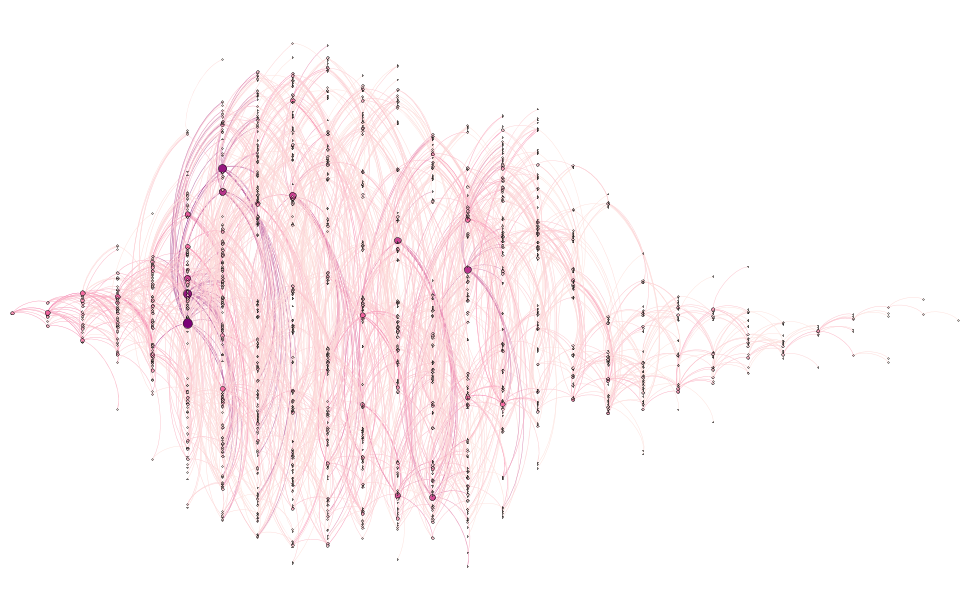
\includegraphics[scale=0.5]{Untitled.png}
 % Untitled.png: 969x591 pixel, 72dpi, 34.18x20.85 cm, bb=0 0 969 591
\end{figure}


\section{Conclusão}

\end{document}
